\documentclass[12pt,a4paper]{article}
\usepackage{graphicx}
\usepackage{ctex}
\usepackage{subfig}
%\usepackage{caption}
\usepackage{bicaption}%属于caption的扩展包,有中英文双语

\usepackage[left=2cm,right=2cm,top=2cm,bottom=2cm]{geometry}

\graphicspath{{Figure/}} %与.tex文件处于同级文件夹

\linespread{1.5}

\captionsetup[figure][bi-second]{name=Fig.}%设置英文图开头为Figure
\captionsetup{labelsep=space}%原本是“图:”的格式,现在将冒号改成空格


\author{Jacob}
\title{图与子图}

\begin{document}

\maketitle

\section{图}

交叉引用,需要引用添加的标签,如:见图\ref{a good figure}。

\begin{figure}[!htbp]
  \centering %居中
  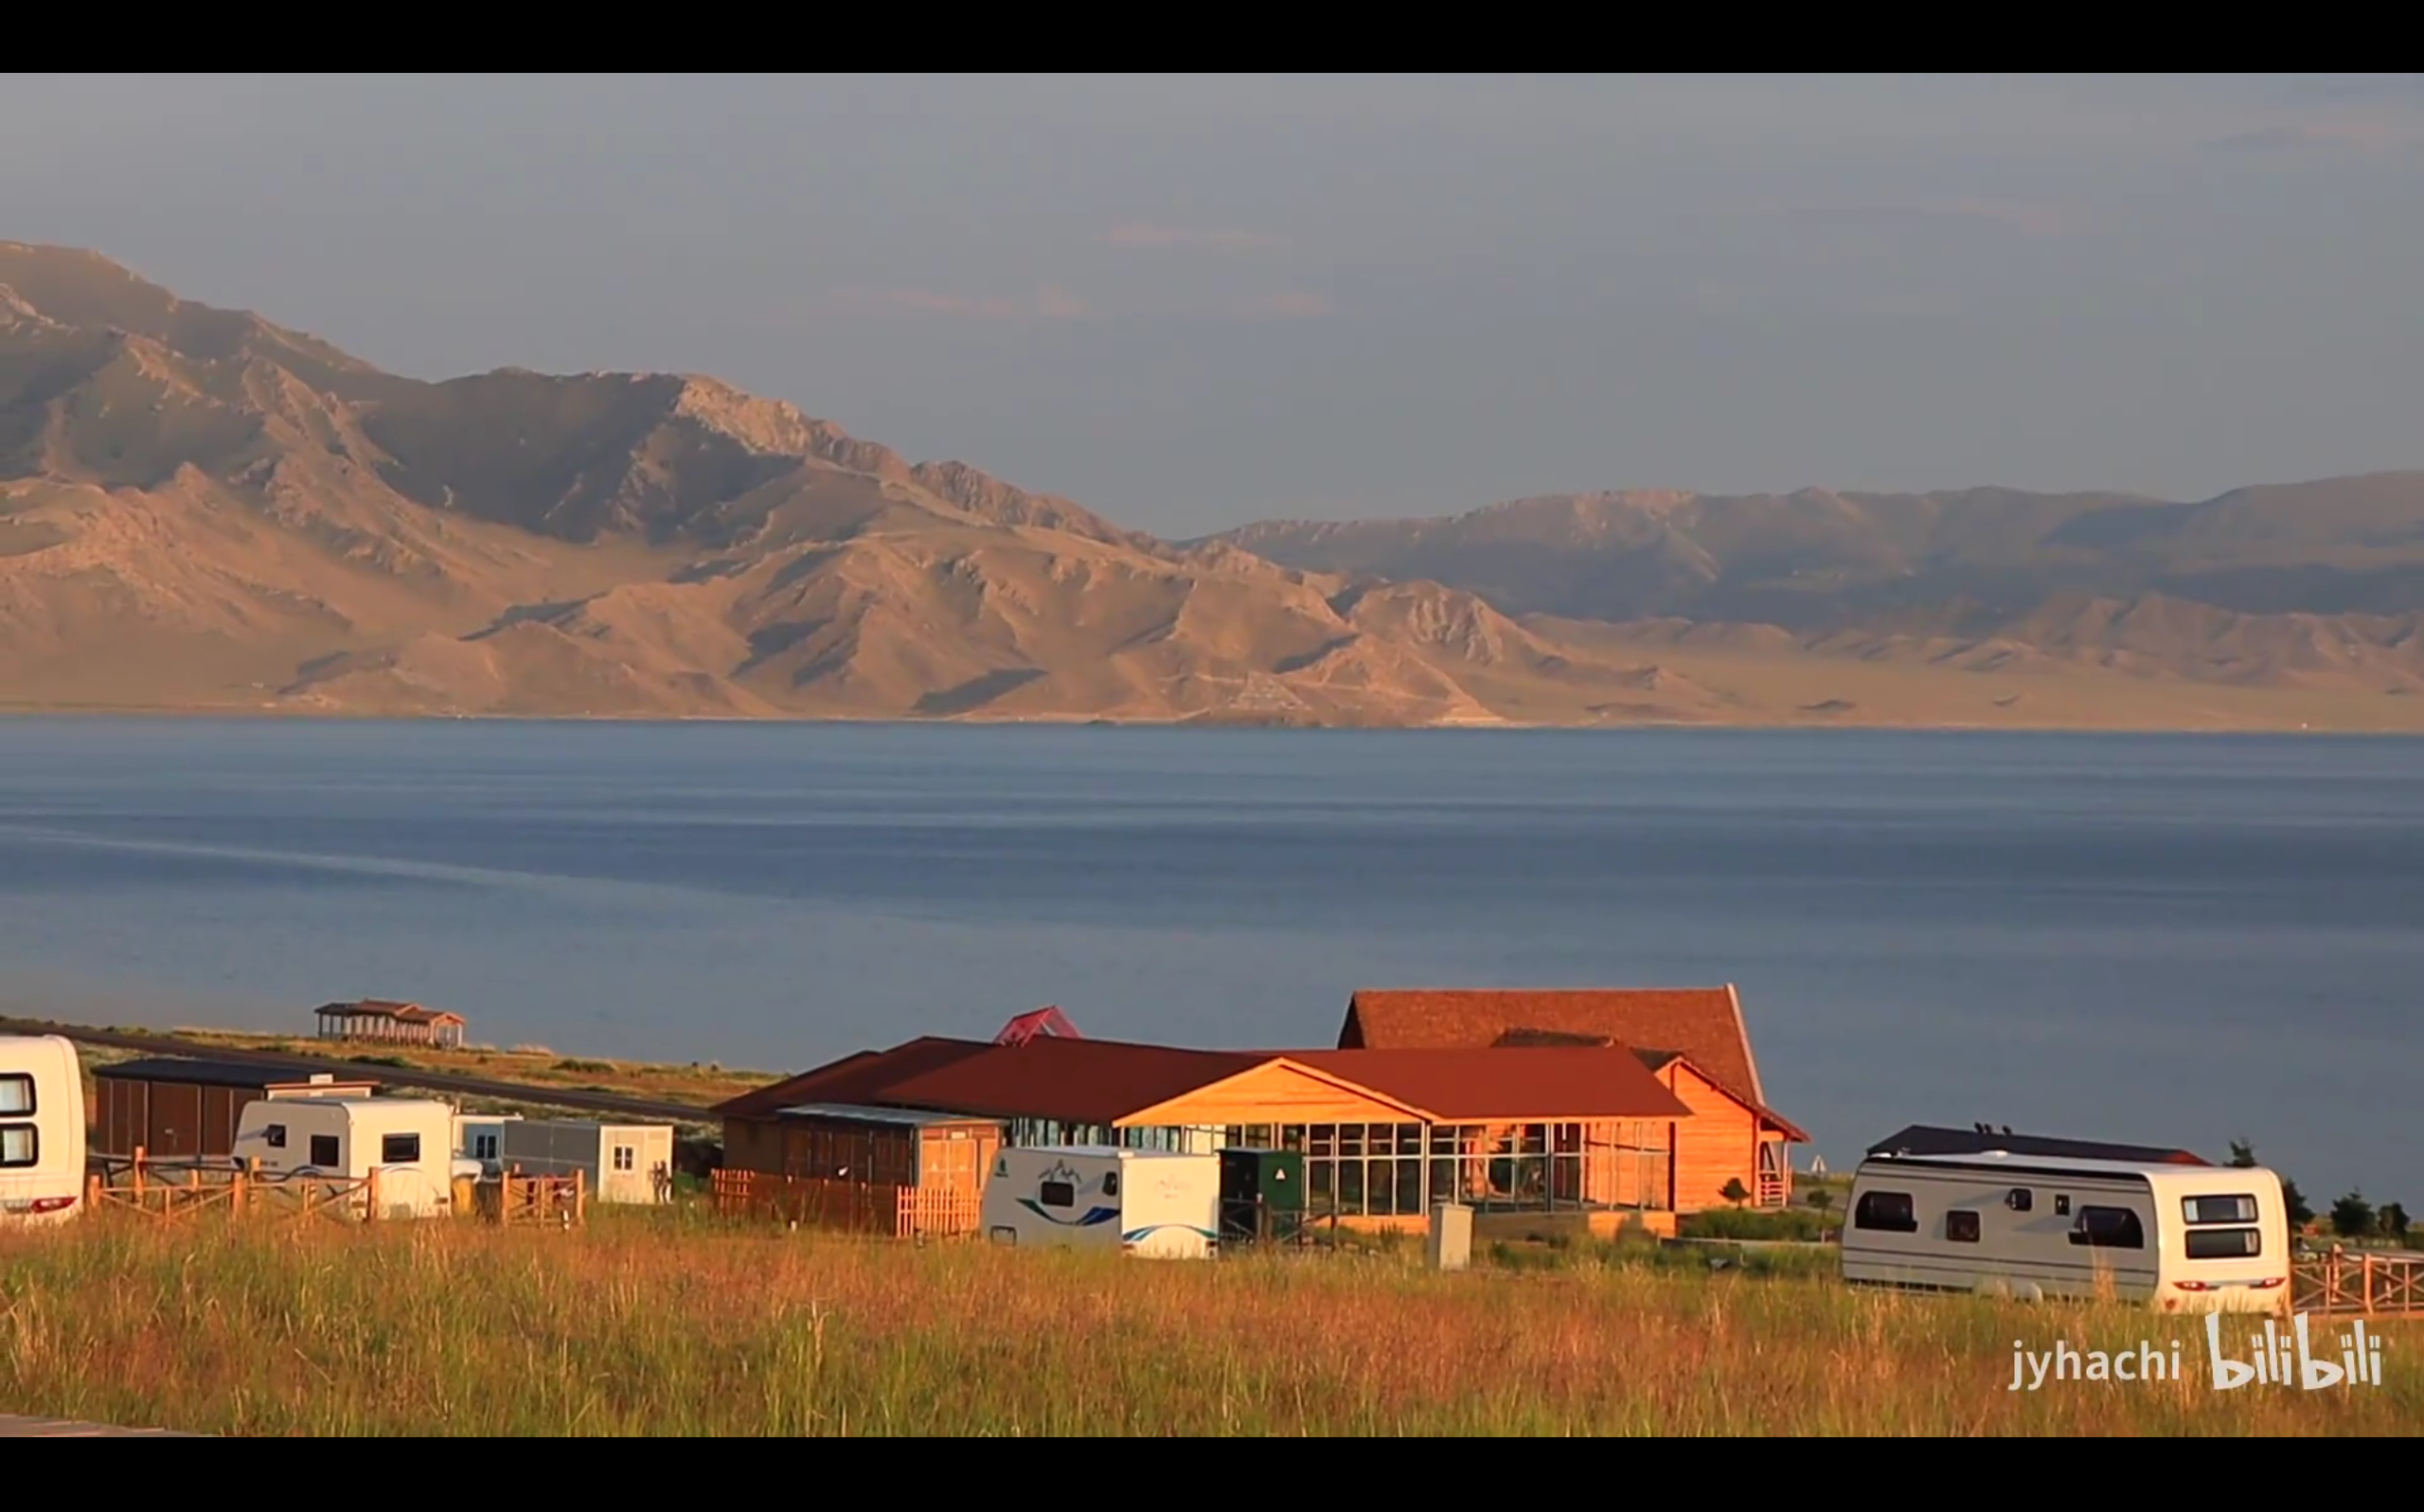
\includegraphics[width=0.6\textwidth]{fig\jinyue.png}%后缀名可省略,图片命名不要带空格不要出现中文,单词可用_分开以识别.[]中括号中的参数很多,我这里只选了宽度
  \caption{一张好图}
  \label{a good figure}%添加标签,标签应方便识别且简洁,供交叉引用
\end{figure}
%[!htbp]
%h	Place the float here, i.e., approximately at the same point it occurs in the source text (however, not exactly at the spot)
%t	Position at the top of the page.
%b	Position at the bottom of the page.
%p	Put on a special page for floats only.
%!	Override internal parameters LaTeX uses for determining "good" float positions.

两张并排,效果如下。
\begin{figure}[!htbp]
  \centering
  \begin{minipage}[h]{0.45\textwidth}
  \centering
  
\includegraphics[width=0.8\textwidth]{fig/hainan.png}%这里的图片宽度是相对于子页的
  \caption{一张极好图}
  \label{a very good figure}%添加标签,供交叉引用
  \end{minipage}
  \quad
  \begin{minipage}[h]{0.45\textwidth}
  \centering
  
\includegraphics[width=0.8\textwidth]{fig/hainan.png}
  \caption{一张奇好图}
  \label{an excellent good figure}%添加标签,供交叉引用
  \end{minipage}
\end{figure}

\section{子图}

在论文中经常有一个figure内含有其他小的figure,这时就要使用一些宏包。
subfigure是比较老的了,目前通用的是subfig,基本上好的主流的国外期刊都会具体要求使用该包。

\subsection{子图仅编号}

看看两种交叉引用的效果,第一种引用子图时一般见图\ref{Fig:P1},第二种引用整图时一般见图\ref{Fig:P12}。

\begin{figure}[!htbp]
	\centering
	\subfloat[]{\label{Fig:P1}%
    
\includegraphics[width=0.45\textwidth]{fig/hainan.png}}
    \quad
    \subfloat[]{\label{Fig:P2}%
    
\includegraphics[width=0.45\textwidth]{fig/hainan.png}}
    
    \caption{两张好图:\protect\subref{Fig:P1}第一张,\protect\subref{Fig:P2}第二张}%这行命令很关键
    \label{Fig:P12}
\end{figure}

\subsection{子图带题注}

只需要将上面的subfloat[]{}中的中括号[]输入子题注内容,即可,效果如下,取决于自己。
\begin{figure}[!htbp]
	\centering
	\subfloat[子题注1]{\label{Fig:F1}%
    
\includegraphics[width=0.45\textwidth]{fig/hainan.png}}    
    \quad
    \subfloat[子题注2]{\label{Fig:F2}%
    
\includegraphics[width=0.45\textwidth]{fig/hainan.png}}
    
    \caption{两张好图}
    \label{Fig:F12}
\end{figure}

\subsection{子页配合排版}

如果一些子图的题注很长,我们就需要使用子页配合排版。

\begin{figure}[!htbp]
	\centering
	\subfloat[子题注1如果一些子图的题注很长,我们就需要使用子页配合排版]{\label{Fig:G1}%
	\begin{minipage}[h]{0.45\textwidth}
	\centering
    \includegraphics[width=\textwidth]{subf3.eps}   %这里的图片宽度是相对于子页的
    \end{minipage}
    }
    \quad
    \subfloat[子题注2基本上好的主流的国外期刊都会具体要求使用该包]{\label{Fig:FG2}%
    \begin{minipage}[h]{0.45\textwidth}
	\centering
    \includegraphics[width=\textwidth]{subf4.eps}
    \end{minipage}
    }
    \caption{又两张好图}
    \label{Fig:FG34}
\end{figure}

\section{中英文双题注}

一般的学位论文以及较为核心的中文期刊中,需要给图形或表格等浮动对象加上双语说明,见图\ref{a good figure with two caption}。
\begin{figure}[!htbp]
  \centering 
  
\includegraphics[width=0.6\textwidth]{fig/hainan.png}
  \bicaption{一张好图含双题注}{A good figure with two caption}
  \label{a good figure with two caption}%添加标签,供交叉引用
\end{figure}


\listoffigures

\end{document}